\documentclass[twocolumn,10pt]{article}
\usepackage[l2tabu,orthodox]{nag}
\usepackage[utf8x]{inputenc}
\usepackage[british]{babel}
\usepackage{microtype}
\usepackage{amsmath}
\usepackage[all]{onlyamsmath}
\usepackage{newtxtext}
\usepackage{newtxmath}
\usepackage[caption=false]{subfig}
\usepackage{booktabs}
\usepackage{upquote}
\usepackage{graphicx}
\usepackage{url}
\usepackage{algorithm}
\usepackage{algpseudocode}
\usepackage{color}
\usepackage[cm]{fullpage}

\frenchspacing
\uchyph=0

\newcommand{\todo}[1]{\textbf{\textcolor{red}{To do: #1}}}
\newcommand{\pb}[1]{\vspace{0.75ex}\noindent{\textbf{#1}}}

%==================================================================================================
\begin{document}

\title{An Empirical Analysis of the Internet Engineering Task Force 
       with Computational Methods}
\author{Colin Perkins\\University of Glasgow}
\maketitle
%==================================================================================================
\begin{abstract}
  % Four sentences:
  %  - State the problem
  %  - Say why it's an interesting problem
  %  - Say what your solution achieves
  %  - Say what follows from your solution

  The Internet requires interoperability between networks, systems, and
  applications, as well as cooperation among a growing number of
  stakeholders. The Internet Engineering Task Force (IETF) is critical in
  supporting this cooperation and interoperability by bringing together
  interested parties and standardising the protocols that power the
  Internet, such as IPv4/6 or HTTP/s. Our work covers more 20 years of IETF
  data, and analyses the participants of the IETF, the emails they
  exchange, and the documents they produce. We show how these data can be
  used to understand who are these Internet actors, and their interests as
  well as how Internet's growth and maturity has given rise to a longer and
  complex standardisation process where participants gain and exercise
  influence and how this is reflected in the language they use and the
  interactions they have.
  

\end{abstract}
%==================================================================================================
\section{Introduction}

% A good paper introduction is fairly formulaic. If you follow a simple set
% of rules, you can write a very good introduction. The following outline can
% be varied. For example, you can use two paragraphs instead of one, or you
% can place more emphasis on one aspect of the intro than another. But in all
% cases, all of the points below need to be covered in an introduction, and
% in most papers, you don't need to cover anything more in an introduction.
%
% Paragraph 1: Motivation. At a high level, what is the problem area you
% are working in and why is it important? It is important to set the larger
% context here. Why is the problem of interest and importance to the larger
% community?



% Paragraph 2: What is the specific problem considered in this paper? This
% paragraph narrows down the topic area of the paper. In the first
% paragraph you have established general context and importance. Here you
% establish specific context and background.



% Paragraph 3: "In this paper, we show that...". This is the key paragraph
% in the introduction - you summarize, in one paragraph, what are the main
% contributions of your paper, given the context established in paragraphs
% 1 and 2. What's the general approach taken? Why are the specific results
% significant? The story is not what you did, but rather:
%  - what you show, new ideas, new insights
%  - why interesting, important?
% State your contributions: these drive the entire paper.  Contributions
% should be refutable claims, not vague generic statements.

In this paper, we ...

% Paragraph 4: What are the differences between your work, and what others
% have done? Keep this at a high level, as you can refer to future sections
% where specific details and differences will be given, but it is important
% for the reader to know what is new about this work compared to other work
% in the area.



% Paragraph 5: "We structure the remainder of this paper as follows." Give
% the reader a road-map for the rest of the paper. Try to avoid redundant
% phrasing, "In Section 2, In section 3, ..., In Section 4, ... ", etc.

We structure the remainder of this paper as follows.

%==================================================================================================
\section{Background and Datasets}

% The following is from our IMC 2021 paper:

We start by presenting an overview of the IETF, and the publication process
for RFCs, before outlining the data sources we use within this paper. We
also highlight the ethical considerations of accessing and processing this
data.


%--------------------------------------------------------------------------------------------------
\subsection{An IETF Primer}

% The following is from our IMC 2021 paper:

\pb{The IETF} is an open standards organisation, which develops
Internet standards via contributions and collaborations across a number of
voluntary stakeholders, including academics, consultants, industry
representatives, governments, and civil society organisations.  Through
extensive collaboration across contributors, the IETF, and associated
organisations, develops Internet standards and other documents. These are
published by the RFC Editor (\url{https://www.rfc-editor.org}) in four
\emph{publication streams}: the IETF stream, the Internet Research Task
Force (IRTF) stream, the Internet Architecture Board (IAB) stream, and the
Independent Submission stream.

There is also a fifth, legacy stream, comprising RFCs published prior to
the adoption of separate publication streams in July 2007 \cite{rfc4844}.
While the IETF is an open standards forum that develops technical standards
and operational guidelines for the Internet, the IRTF is an associated
organisation that promotes longer-term research, and the IAB provides
long-range technical direction for Internet development. The Independent
Submission stream ``allows RFC publication for some documents that are
outside the official IETF/IAB/IRTF process but are relevant to the Internet
community'' (\url{https://www.rfc-editor.org/about/independent}).

\pb{The standards development process} is an inherently collaborative
activity.  Most day-to-day work is conducted on public mailing lists, in
conjunction with three plenary meetings and numerous interim working group
meetings per year. 
The mailing lists are broadly split into three categories: announcement
lists, where replies are not allowed; non-working group lists, for
discussing topics that do not relate to the work within an IETF working
group or IRTF research group; and working group and area lists, where
technical discussions take place.

The process of RFC publication begins with the submission of an
\emph{Internet-Draft}. Whereas anyone can post a draft, not all drafts
become RFCs. After a draft is first posted, multiple revisions might take
place resulting in multiple versions of the draft. Each new draft is
announced on one or more mailing lists related to the topic of the draft,
soliciting feedback and encouraging discussion. Drafts are initially posted
by individuals. For publication under the IETF stream, drafts must then be
adopted by a working group, where, via further revision, the draft may
ultimately be published as an RFC. The process of managing drafts, and the
degree and type of peer review conducted prior to their submission to the
RFC Editor for publication, differs between streams.

Once the technical development of the draft is complete its publication is
managed by the RFC Editor, who maintains the master archive of the RFC
documents, along with an index of metadata pertaining to the RFCs and their
authors. Finally, once an RFC has been published, deployment is voluntary,
and therefore not all RFCs are widely implemented.

%--------------------------------------------------------------------------------------------------
\subsection{Data Sources}


%--------------------------------------------------------------------------------------------------
\subsection{Ethical Considerations}
\label{sec:ethics}

% The following is from our IMC 2021 paper:

The data we analyse is extracted from public IETF archives and APIs.  We
have taken steps to ensure ethical compliance.  To ensure that our access
to these services does not cause operational problems for the IETF, we are
in regular contact with the IETF Tools Team and Secretariat, as well as the
operators of the Datatracker and mailing list archive.  We have extensively
discussed our work with IETF leadership (IETF and IAB Chairs, the IETF
Executive Director, and the IRTF Chair, who is a co-author on this paper)
to ensure that our access falls within their acceptable use policies.

Participation in the IETF is dependent on agreement to abide by the
policies and procedures described at \url{https://www.ietf.org/about/note-well},
including the privacy policy at \url{https://www.ietf.org/privacy-statement}.
These make explicit provision that mailing list archives and the metadata
contained in the Datatracker system will be made public, and it is this
public data that we process to extract the aggregate statistics presented
in Sections \ref{sec:documents}, \ref{sec:authors}, and \ref{sec:mail}, as
well as the features analysed in Section \ref{sec:model}. We transfer and
store data securely, and retain it only for the time needed to perform the
analysis.  Since we operate entirely using the public APIs provided by
IETF, we have no access to private data about individuals.

In balancing these ethical considerations with the reproducibility of our
work, we provide the tools needed to access the datasets from the relevant
IETF sources, rather than the data itself.


%==================================================================================================
\section{Trends in RFC Publication}

% \begin{figure}
%   \centering
%   \includegraphics{figures/rfcs-by-year-stream.pdf}
%   \caption{Number of RFCs published per year}
%   \label{fig:rfcs-by-year}
% \end{figure}


%--------------------------------------------------------------------------------------------------
\subsection{Document Production and Complexity}

% The following is from our IMC 2021 paper, Section 3.1:

\pb{Growth of RFCs.}
In total, 8,711 RFCs have been published through to the end of 2020.
Figure~\ref{fig:rfcs_by_area} shows how publication trends, in terms of
IETF areas and non-IETF streams, have changed over time. We identify three
broad publication phases in the RFC series. First, in 1969 through 1974,
RFCs are published at a rapid rate during the initial development of the
ARPANET. Then, from 1975 through 1985, development slows. This reflects a
relatively small community that is gaining real-world experience with the
network and developing a small core of applications and protocols. Finally,
with the creation of the IETF and the introduction of the National Science
Foundation Network (NSFNET) in 1986, both the community, and the number of
RFCs published, starts to expand rapidly. This is further driven by the
opening of the network to commercial and public use in the mid-1990s, and
continues to this day.

As shown, the annual RFC publication rate was highest in 2005, at the peak of
the standardisation efforts for SIP and related standards for voice-over-IP and
Internet telephony. The rate of publication has slowed in recent years,
following the completion of large work programmes relating to HTTP/2 and WebRTC.

\begin{figure}
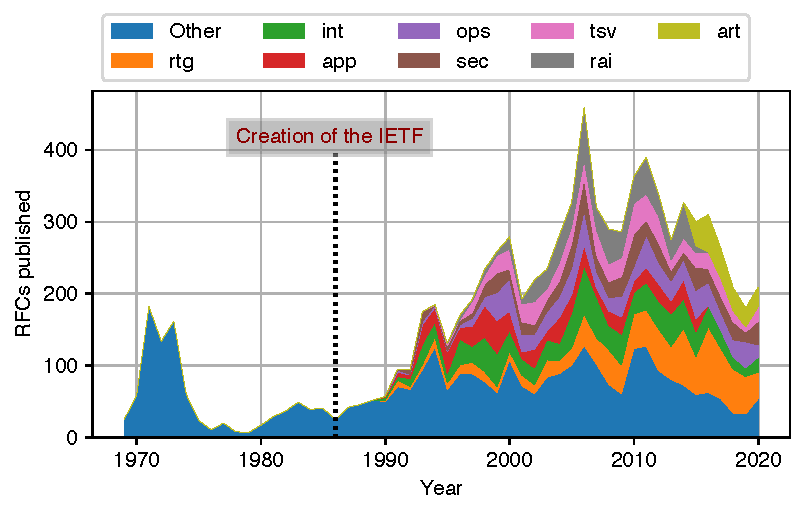
\includegraphics[width=0.45\textwidth]{figures-prev/imc-2021/documents/rfcs_areas.pdf}
\caption{RFCs by area. \textit{Other} includes legacy RFCs, and RFCs from other non-IETF streams.}
\label{fig:rfcs_by_area}
\end{figure}


\pb{Role of Working Groups (WGs).}
From the creation of the IETF in 1986, the growing community with its interests
in an increasing set of applications and protocols, has been split into working
groups. These working groups are chartered with a focus on a well-defined
programme of work, and exist within areas that have a broader focus.
As shown in
Figure~\ref{fig:rfcs_by_area}, the output of different areas has remained
relatively stable over time. The most notable trends begin with the creation of
the Real-time Applications and Infrastructure (rai) area from within the
Transport (tsv) area, and its later merger with the Applications (app) area to
become the Applications and Real-Time (art) area around 2014. Additionally, we also observe the significant growth in output of the Routing (rtg) area,
owing to the ongoing development of standards for MPLS, service function
chaining, and fat tree routing in data centres.

To give a sense for the broader productivity of the IETF,
Figure~\ref{fig:pub_wgs_yearly} shows the number of working groups that
publish RFCs each year. This highlights how the structure of the IETF has
grown to accommodate its larger community: in the early 1990s, fewer than
20 working groups were actively publishing RFCs, while in recent years
there has typically been at least 60 different publishing groups, with a
peak of 97 active working groups, and other activities, in 2011.

\begin{figure}
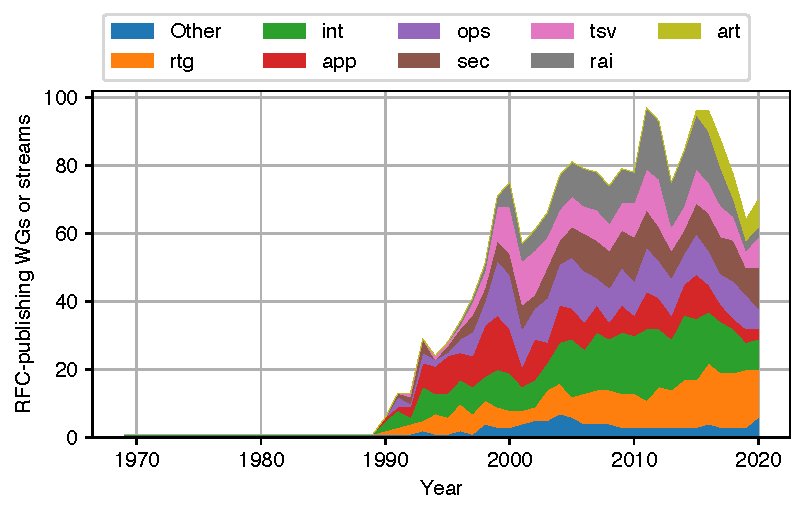
\includegraphics[width=0.45\textwidth]{figures-prev/imc-2021/documents/unique_wgs_per_year_areas.pdf}
\caption{Number of publishing working groups. \textit{Other} includes legacy RFCs, IRTF research groups, and non-IETF streams.}
\label{fig:pub_wgs_yearly}
\end{figure}

Figure~\ref{fig:rfcs_days_to_pub} plots the median number of days from the
submission of an RFC's first draft, through to its publication as an RFC.
This shows a clear trend: RFCs are taking longer to make their way through
the standardisation and publication process. The median number of days to
publication was 469 in 2001, rising to 1,170 in 2020. Further,
Figure~\ref{fig:drafts_year} shows the median number of Internet-Drafts
that are posted before an RFC is published. Days to publication and number
of drafts are strongly correlated, suggesting that the time is spent making
changes to the document. This may go some way towards explaining the
decline in output of the IETF: each RFC is taking longer to produce, with
more revisions before publication. 

\begin{figure}
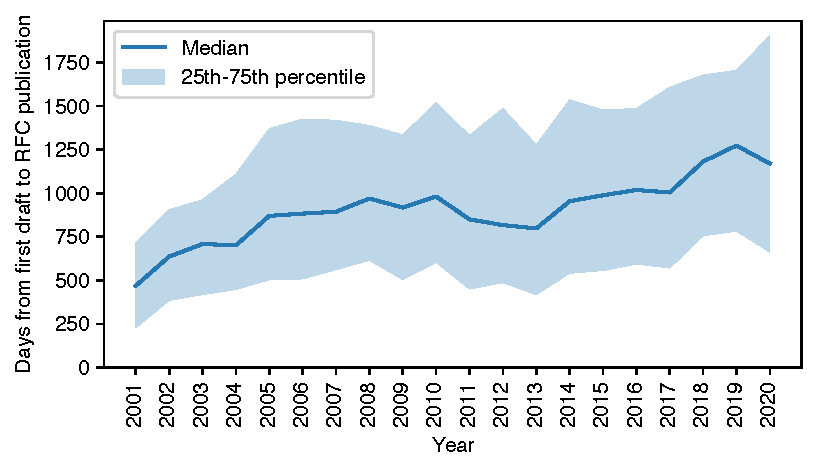
\includegraphics[width=0.45\textwidth]{figures-prev/imc-2021/documents/day_counts_yearly.pdf}
\caption{Days from first draft to RFC publication}
\label{fig:rfcs_days_to_pub}
\end{figure}

\begin{figure}
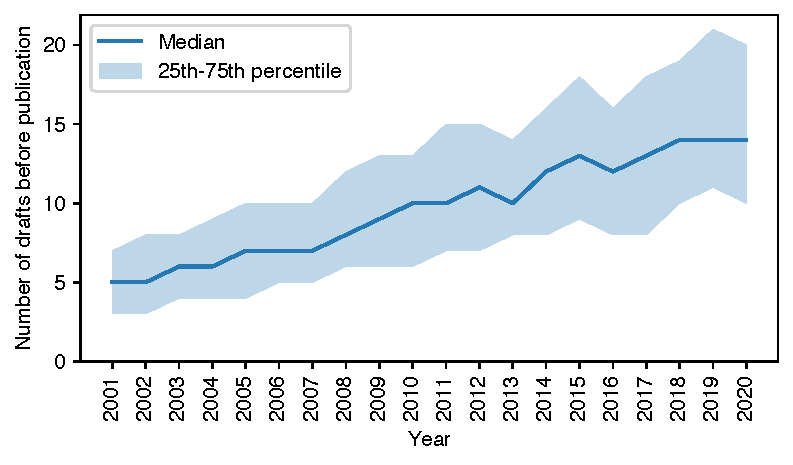
\includegraphics[width=0.45\textwidth]{figures-prev/imc-2021/documents/draft_counts_yearly.pdf}
\caption{Number of drafts per RFC}
\label{fig:drafts_year}
\end{figure}

\pb{RFC Length.}
One may conjecture that this slowdown is driven by longer RFCs that contain
more material. To explore this, Figure~\ref{fig:pages_year} shows the
median page count of RFCs. This shows that the increase in the duration of
the standardisation process for RFCs cannot be attributed to RFCs becoming
longer: median page counts have remained stable. 

\begin{figure}
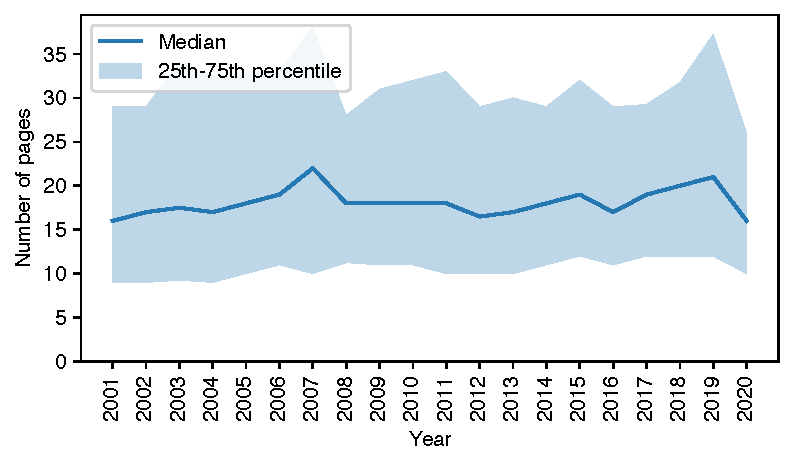
\includegraphics[width=0.45\textwidth]{figures-prev/imc-2021/documents/page_counts_yearly_dt.pdf}
\caption{RFC page counts}
\label{fig:pages_year}
\end{figure}

\pb{Relationships between RFCs.}
RFCs themselves may be becoming more complex as a result of them needing to
describe their relationship with older standards. As the Internet has
evolved and matured, applications and protocols must be maintained, and new
standards need to interoperate with existing RFCs.
Figure~\ref{fig:updates_year} highlights this, showing the proportion of
RFCs that are published each year that update (i.e., extend or augment) or
obsolete (i.e., replace) one or more previously published RFCs. Intuitively,
this percentage has slowly increased as the IETF has matured: in 2020, more
than 30\% of RFCs updated or made obsolete a previous RFC.
Figure~\ref{fig:citations_year} expands on this, showing the median number
of citations from each RFC to other Internet-Drafts and RFCs. This
similarly shows that RFCs are increasingly referring to prior work.

\begin{figure}
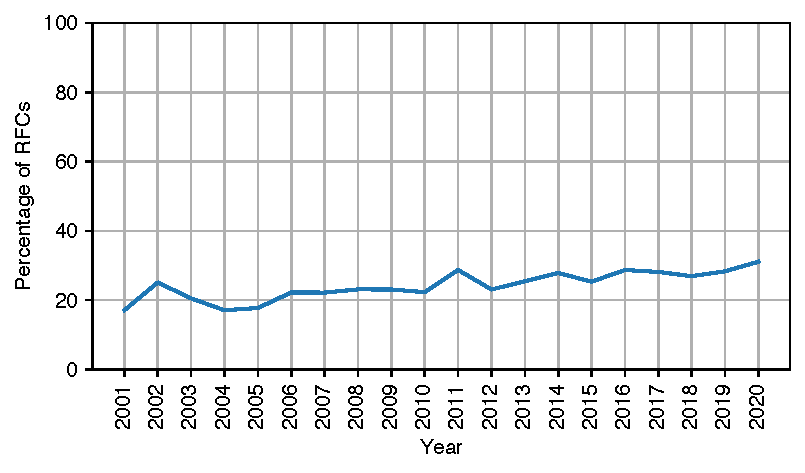
\includegraphics[width=0.45\textwidth]{figures-prev/imc-2021/documents/update_obsolete_yearly_pct.pdf}
\caption{RFCs that update or obsolete previous RFCs}
\label{fig:updates_year}
\end{figure}

\begin{figure}
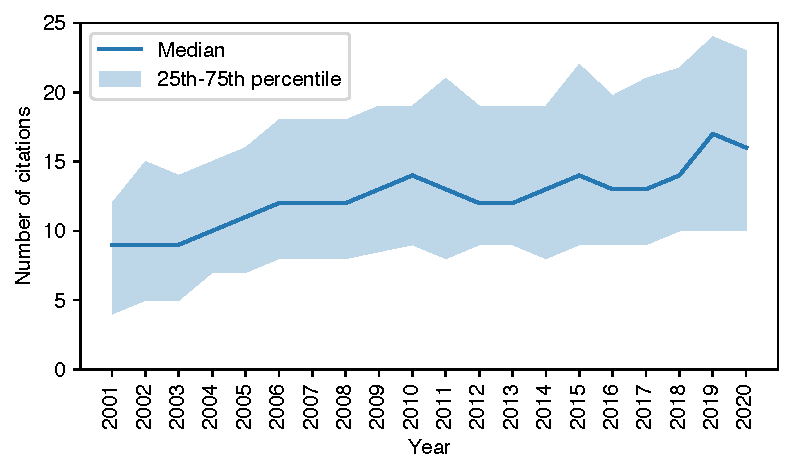
\includegraphics[width=0.45\textwidth]{figures-prev/imc-2021/documents/cite_counts_yearly.pdf}
\caption{Citations from RFCs to other Internet-Drafts and RFCs per RFC}
\label{fig:citations_year}
\end{figure}

\pb{Use of requirements-setting language.}
Figure~\ref{fig:keyword_usage_rates} further confirms the growing
complexity of RFCs, showing how the use of keywords has evolved over time.
Keywords are used in RFCs to indicate the normative requirements an RFC
imposes on implementations. Figure~\ref{fig:keyword_usage_rates} shows the
total number of occurrences of each of the RFC 2119~\cite{RFC2119} keywords
(i.e., MUST, MUST NOT, REQUIRED, SHALL, SHALL NOT, SHOULD, SHOULD NOT,
RECOMMENDED, MAY, OPTIONAL), divided by the page count of the RFC. As
shown, the median number of keywords per page grew from 2001 through to
2010, indicating a growing number of requirements being expressed in RFCs,
before plateauing in recent years.

\begin{figure}
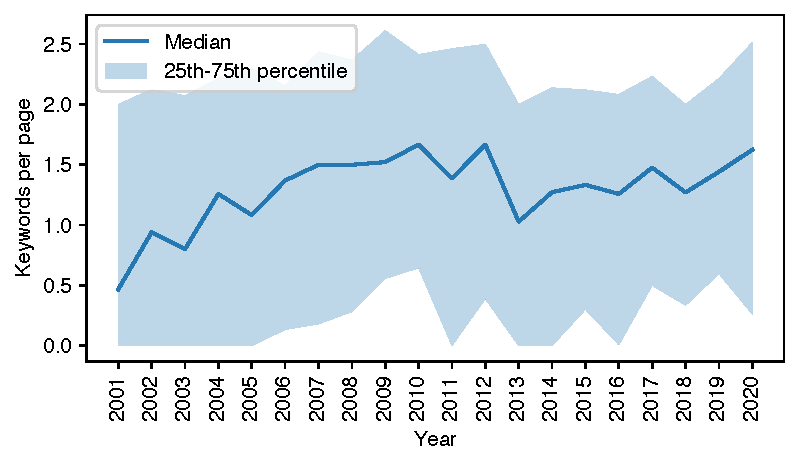
\includegraphics[width=0.45\textwidth]{figures-prev/imc-2021/documents/keyword_usage_rate.pdf}
\caption{Keyword occurrences per page}
\label{fig:keyword_usage_rates}
\end{figure}


\todo{Should we include ``Academic impact of RFCs'' from IMC 2021?}


\pb{Summary.}
RFCs are taking longer to produce, and they go through a greater number of
revisions before publication. Further, they increasingly update or
reference previously published RFCs, and make greater use of
requirements-setting keywords. Yet, while these measures indicate that the
overall complexity of standards documents is increasing, none of these
factors strongly correlate with the time taken to publish RFCs. This
indicates that these factors aren't driving the increasing duration of the
standardisation process. In the sections that follow, we explore trends in
authorship and community interaction that may also impact the process.


%--------------------------------------------------------------------------------------------------
\subsection{Document Errata}

% The following is from our TMA 2023 paper, Section III:

\pb{Errata over Time.}
Figure~\ref{fig:errata_per_year} presents the number of errata filed, on
average per RFC, since 1969 based on the year of RFC publication.  The peak
in the number of errata per RFC occurs in 1981. Only 29 RFCs were published
that year, but they include major documents such as RFCs 791, 792, and 793
(the original versions of the IP~\cite{rfc791}, ICMP~\cite{rfc792}, and
TCP~\cite{rfc793} standards), with 17, 7, and 47 errata, respectively.
These important protocols clearly garnered a great deal of scrutiny and
revision.  The second highest peak occurs in 2006.  In contrast to the
previous examples, this has the highest number of RFCs published per year
(459), including RFC 4601 \cite{RFC4601} that has the most errata (114).
Since this second peak, there has been a steady decrease in the number of
errata filed.  This broadly correlates with the number of RFCs published
per year, with Pearson coefficient 0.59 since 2007.  Table
\ref{tab:top-10-rfcs-by-errata} lists the top RFCs by errata filing count.

\begin{figure}
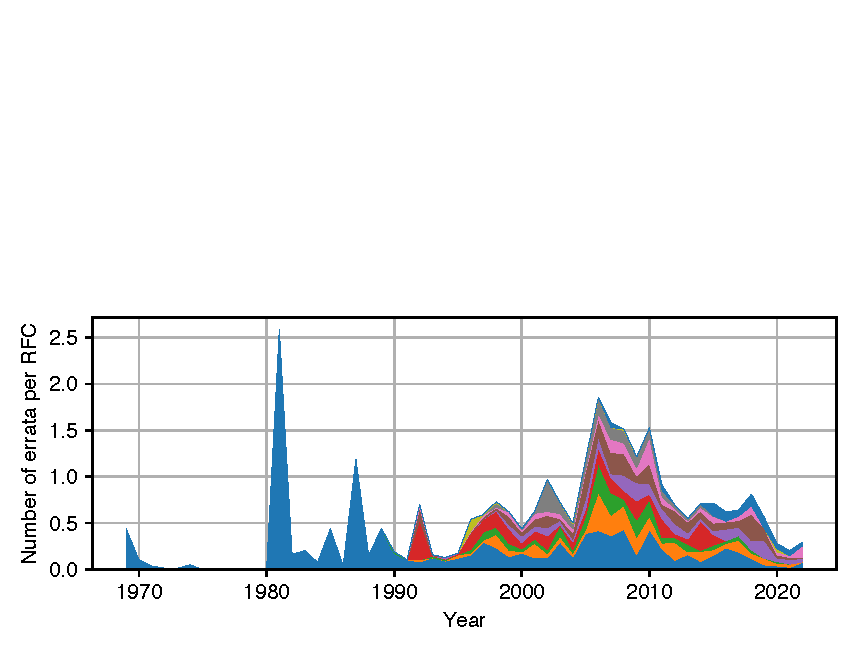
\includegraphics[width=0.45\textwidth]{figures-prev/tma-2023/errata-by-year.pdf}
\caption{Average errata filed per RFC for each year by RFC publication year,
grouped by IETF area (acronyms expanded in Table~\ref{tab:errata-stats-area}).}
\label{fig:errata_per_year}
\end{figure}

\begin{table*}
\centering
\footnotesize
\begin{tabular}{rlrrr}
\toprule
\textbf{RFC} & \textbf{Title} & \textbf{Year} & \textbf{Area} & \textbf{Filing count} \\
\midrule
4601 & Protocol Independent Multicast - Sparse Mode (PIM-SM): Protocol Specification (Revised) & 2006 & rtg & 114 \\
4880 & OpenPGP Message Format & 2007 & sec & 52 \\
793 & Transmission Control Protocol & 1981 & None & 47 \\
4634 & US Secure Hash Algorithms (SHA and HMAC-SHA) & 2006 & None & 44 \\
5661 & Network File System (NFS) Version 4 Minor Version 1 Protocol & 2010 & tsv & 42 \\
1345 & Character Mnemonics and Character Sets & 1992 & app & 41 \\
8446 & The Transport Layer Security (TLS) Protocol Version 1.3 & 2018 & sec & 40 \\
5545 & Internet Calendaring and Scheduling Core Object Specification (iCalendar) & 2009 & app & 35 \\
3261 & SIP: Session Initiation Protocol & 2002 & rai & 33 \\
5905 & Network Time Protocol Version 4: Protocol and Algorithms Specification & 2010 & int & 32 \\
\bottomrule
\end{tabular}
\caption{Top 10 RFCs by errata filing count}
\label{tab:top-10-rfcs-by-errata}
\end{table*}

\begin{table*}
\centering
\footnotesize
\begin{tabular}{lr|rrrr|rr}
\toprule
\textbf{Area} & \textbf{\#} & \textbf{Verified} & \textbf{Held} & \textbf{Rejected} & \textbf{Reported} & \textbf{Technical} & \textbf{Editorial} \\
\midrule
None & 1883  & 895  & 505  & 197  & 286  & 930  & 953 \\
Internet (int) & 650  & 281  & 223  & 98  & 48  & 342  & 308 \\
Operations and Management (ops) & 558  & 311  & 113  & 67  & 67  & 297  & 261 \\
Real-time Applications and Infrastructure (rai) & 457  & 143  & 213  & 48  & 53  & 255  & 202 \\
Security (sec) & 888  & 291  & 265  & 115  & 217  & 447  & 441 \\
Routing (rtg) & 831  & 305  & 378  & 140  & 8  & 326  & 505 \\
Applications (app) & 787  & 370  & 175  & 116  & 126  & 464  & 323 \\
Transport (tsv) & 459  & 188  & 142  & 75  & 54  & 258  & 201 \\
General (gen) & 41  & 22  & 4  & 5  & 10  & 8  & 33 \\
Applications and Real-Time (art) & 204  & 64  & 32  & 16  & 92  & 143  & 61 \\
Sub-IP (subip) & 1  & 1  & 0  & 0  & 0  & 1  & 0 \\
\midrule All & 6759  & 2871  & 2050  & 877  & 961  & 3471  & 3288 \\
\bottomrule
\end{tabular}
\caption{Errata statistics by area.}
\label{tab:errata-stats-area}
\end{table*}


\pb{Errata Delay.}
We next explore how long it takes for errata to be identified and filed.
Figure~\ref{fig:errata_submission_days} presents a CDF of the number of
days between RFC publication and the errata being filed, broken down based
on IETF area. We see a wide range of delays. 7.3\% of errata are filed
within the first 30 days, suggesting that many RFCs are published with
issues that could have been identified prior to publication.  RFCs from the
General (\emph{gen}) area--describing IETF policies and procedures--have
the longest delay, with a median of 3,458 days, compared to the
Applications and Real-time (\emph{art}) area with a median of 681
days.\footnote{Errata are filed against RFCs within the \emph{subip} area
within a median of 48 days, but this is skewed, with only 19 RFCs being
published in that area.} Editorial errata are typically filed more quickly,
with a median of 987 days, compared to a median of 1,138 days for technical
errata. 


\begin{figure}
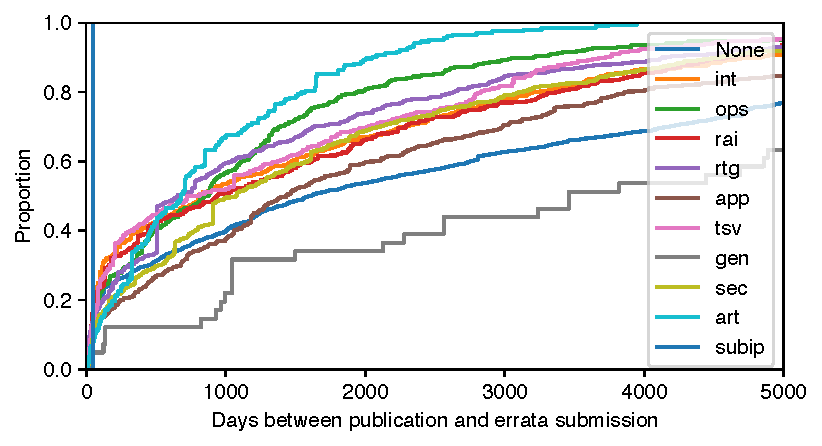
\includegraphics[width=0.45\textwidth]{figures-prev/tma-2023/errata-submission-dates-area.pdf}
\caption{Days from RFC publication and errata filing by IETF area (acronyms
  expanded in Table~\ref{tab:errata-stats-area}).}
\label{fig:errata_submission_days}
\end{figure}


\pb{Errata Status.}
Figure~\ref{fig:errata_status} categorises the errata by status and
publication year of the RFC to which they relate. 

\begin{figure}
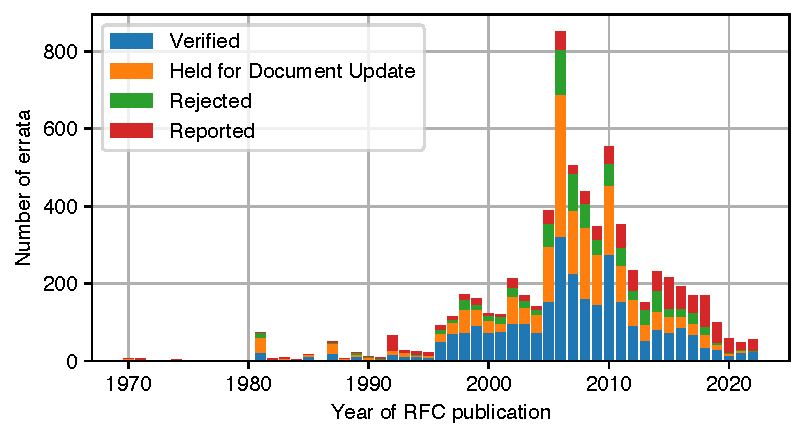
\includegraphics[width=0.45\textwidth]{figures-prev/tma-2023/errata-by-status.pdf}
\caption{Errata filings by status, by publication year of the RFC.}
\label{fig:errata_status}
\end{figure}

The largest share (42.5\%) of errata are \emph{verified}: errata that have
been has been confirmed as necessary and accurate. This suggests that many
errata are useful to the community. The next largest share (30.3\%) are
those labelled \emph{hold for document update}.  These are errata that are
not a necessary update to the RFC, but may be considered on future
revisions. For example, \emph{erratum 6278} describes an oversight in RFC
8610~\cite{rfc8610}; the solution to this is non-trivial, and so will be
considered in the next version of the specification. Of the 930 RFCs that
have \emph{hold for document update} errata filed against them, only 40\%
have been updated or obsoleted by a subsequent RFC.  We flag that this may
be a cause for concern, or at least a missed opportunity for improvements
to standards.

The third largest category (13\%) is \emph{rejected}, which covers errata
that are invalid (like \emph{erratum 6323}, which was rejected because the
original text was understood to be correct) or proposes a significant
change to the RFC that should be done by publishing a new RFC (like
\emph{erratum 5814}, which was rejected for proposing a significant change,
rather than reporting an error). Such a large fraction of rejected
submissions is unexpected and may flag issues with people's understanding
of the errata process and its place within the wider standardisation
process.  Finally, 14.2\% of errata are \emph{reported} but unverified.
Again, we are surprised to see unverified errata from over a decade ago,
suggesting the process should be expedited. 


\pb{Errata per RFC Area, Status, and Stream.}
Figure~\ref{fig:errata_per_rfc} shows a CDF of the number of errata filed,
per RFC, in each IETF area. Non-IETF RFCs, e.g., IRTF and independent stream
RFCs, and legacy IETF RFCs, are labelled as ``None''.  We confirm errata in
standards are common: of the 4,373 standards-track RFCs in our dataset,
32.7\% have attracted at least one erratum filing.  However, there are
three notable outliers.  First, RFCs published by the Sub-IP (subip) Area
have very few errata, with only 5\% of subip RFCs attracting errata
filings. This is because this temporary area -- established in 2001 and
concluded in 2005 -- only published 19 RFCs, resulting in a far smaller
sample than the other areas. For comparison, the next smallest area,
General (gen), published 39 RFCs. \emph{gen} RFCs attract a greater number
of errata on average, vs. \emph{subip} RFCs, likely due to their broader
relevance.  Second, we see that both the Application (app) and Security
(sec) Areas' RFCs are more likely to have errata filed for them, with
35.9\% of Application and 39\% of Security RFCs attracting at least one
erratum filing.

\begin{figure}
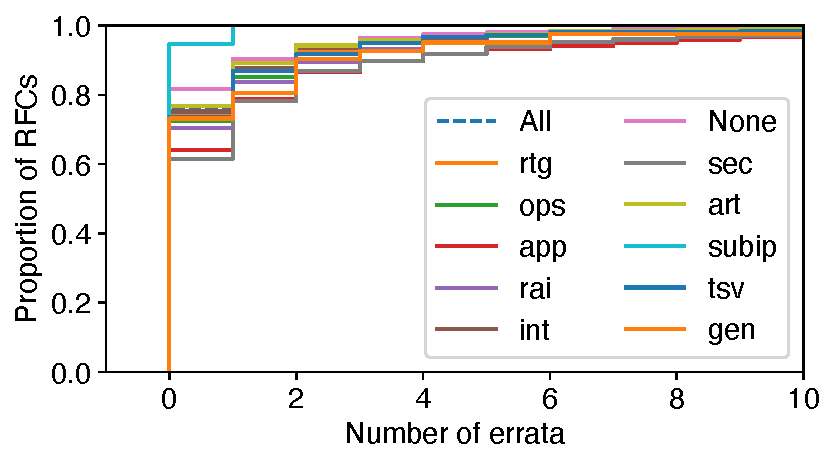
\includegraphics[width=0.45\textwidth]{figures-prev/tma-2023/errata-by-rfc-by-area.pdf}
\caption{CDF of errata filed per RFC by grouped by IETF area (acronyms
  expanded in Table~\ref{tab:errata-stats-area}).}
\label{fig:errata_per_rfc}
\end{figure}

Finally, Table~\ref{tab:errata-stats-area} details the split between
\emph{technical} and \emph{editorial} errata across each area. While there
is broadly an even split, there are areas where one type of errata is more
dominant. For example, in the Routing (rtg) area, 60.8\% of filings are
editorial, while in the Applications (app) area, 59\% were technical.  It
remains to determine why this is the case, and, in particular, to establish
whether there is something inherent about the RFCs published by these areas
that makes them more prone to containing errata, and to containing one type
of errata vs. another. For example, in the Routing area, structured
notation is frequently used to define routing entities; editorial errata
are often filed in those definitions. Targeting such areas with improved
alternate review procedures may be beneficial.

Tables~\ref{tab:errata-stats-stream} and \ref{tab:errata-stats-status}
further categorise errata by the stream and status, at the time of
publication, of each RFC. As expected, the majority of errata are filed
against IETF RFCs and \emph{Proposed Standards} since these make up the
majority of RFCs that are published. However, there are notable differences
in the average number of filings per RFC. \emph{Proposed Standards} (1.01
errata per RFC), \emph{Draft Standards} (1.93), and \emph{Internet
Standards} (2.17) attract a far higher number of errata per RFC than
\emph{Informational} (0.52) or \emph{Experimental} (0.39) documents. This
may be due to the additional readership and attention that standards-track
documents receive, and because they are more likely to be the basis for
future work and protocol extensions.

\begin{table*}
\centering
\footnotesize
\begin{tabular}{lr|rrrr|rr}
\toprule
\textbf{Stream} & \textbf{\#} & \textbf{Verified} & \textbf{Held} & \textbf{Rejected} & \textbf{Reported} & \textbf{Technical} & \textbf{Editorial} \\
\midrule
IETF (6619) & 5797  & 2348  & 1815  & 798  & 836  & 3034  & 2763 \\
IAB (124) & 55  & 25  & 13  & 3  & 14  & 23  & 32 \\
Independent (376) & 330  & 235  & 32  & 28  & 35  & 172  & 158 \\
Legacy (1929) & 510  & 226  & 182  & 39  & 63  & 198  & 312 \\
IRTF (97) & 67  & 37  & 8  & 9  & 13  & 44  & 23 \\
\midrule All & 6759  & 2871  & 2050  & 877  & 961  & 3471  & 3288 \\
\bottomrule
\end{tabular}
\caption{Errata statistics by stream; the ``\emph{Editorial}'' stream has no documents, and is not shown.}
\label{tab:errata-stats-stream}
\end{table*}

\begin{table*}
\centering
\footnotesize
\begin{tabular}{lr|rrrr|rr}
\toprule
\textbf{Status} & \textbf{\#} & \textbf{Verified} & \textbf{Held} & \textbf{Rejected} & \textbf{Reported} & \textbf{Technical} & \textbf{Editorial} \\
\midrule
Proposed Standard (4084) & 4142  & 1680  & 1308  & 555  & 599  & 2213  & 1929 \\
Informational (2894) & 1500  & 719  & 399  & 136  & 246  & 754  & 746 \\
Internet Standard (147) & 319  & 118  & 111  & 66  & 24  & 135  & 184 \\
Best Current Practice (316) & 233  & 111  & 53  & 30  & 39  & 80  & 153 \\
Historic (70) & 20  & 13  & 4  & 2  & 1  & 9  & 11 \\
Draft Standard (142) & 274  & 94  & 93  & 66  & 21  & 150  & 124 \\
Experimental (563) & 221  & 115  & 65  & 20  & 21  & 121  & 100 \\
Unknown (929) & 50  & 21  & 17  & 2  & 10  & 9  & 41 \\
\midrule All & 6759  & 2871  & 2050  & 877  & 961  & 3471  & 3288 \\
\bottomrule
\end{tabular}
\caption{Errata statistics by status at publication.}
\label{tab:errata-stats-status}
\end{table*}


\todo{Should we include ``Impact of Citations'' from TMA 2023?}

\pb{Errata Location.}
Finally, we investigate the location of errata within RFCs.
Figure~\ref{fig:errata_location_percent_count} presents the number of
errata occurring at each decile of the documents, for the 2,552 filings
where accurate location information is available, and after the copyright
notice and other boilerplate has been removed.  We see that technical
errata dominate over editorial in almost all places, except for the very
beginning where the \textit{Introduction} is located. Moreover, it shows
that the most technical errata are near the middle of the document where
the most complex content is.  We explore where errata occur, with
Figure~\ref{fig:errata_section_wise_counts} showing section titles for
errata appearing in at least $10$ documents. Sections such as the
\emph{Introduction} or \textit{References} are dominated by editorial
errata while more technical sections, like \emph{IANA Considerations} (i.e.,
parameter registrations), \emph{Security Considerations} or
\emph{Definitions}, have a larger proportion of technical errata. In
addition, we see that sections labelled \emph{Appendix} attract a
significant proportion of technical errata. While appendices vary in their
content, they are widely used to provide pseudocode and test vectors, or to
describe algorithms. This suggests that it may be useful to target review
efforts on appendices and other dense technical content where errata are
more likely.

\begin{figure}
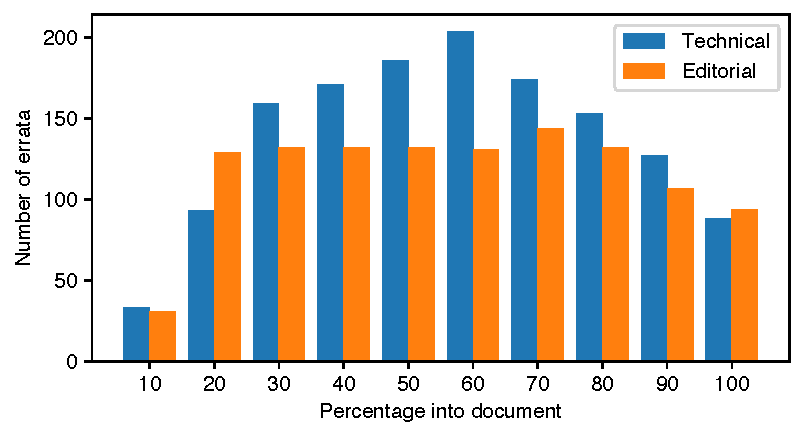
\includegraphics[width=0.45\textwidth]{figures-prev/tma-2023/location-percent.pdf}
\caption{Errata counts by percentile location in document (0 is the beginning; 100 is the end).}
\label{fig:errata_location_percent_count}
\end{figure}

\begin{figure}
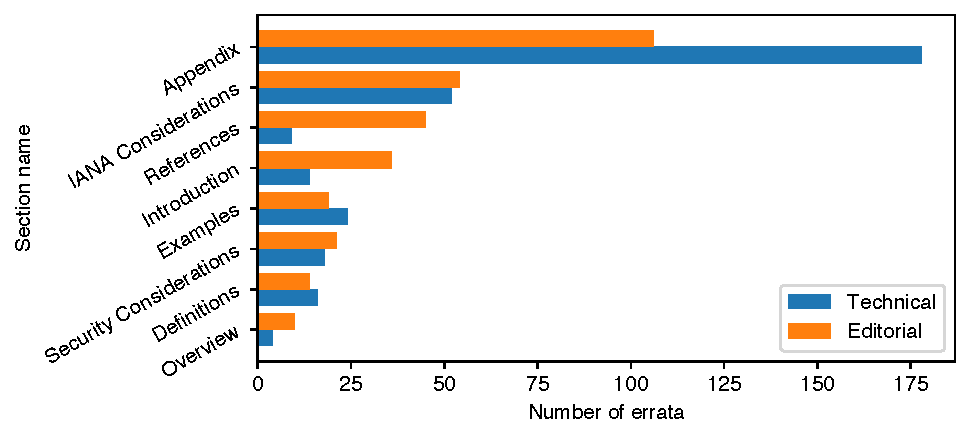
\includegraphics[width=0.45\textwidth]{figures-prev/tma-2023/section-title-counts.pdf}
\caption{Errata counts by section title for the more frequent section titles.}
\label{fig:errata_section_wise_counts}
\end{figure}

%==================================================================================================
\section{Exploring Authorship}




%==================================================================================================
\section{Related Work}

% This should come near the end, and focussing on discussing how your work
% relates to that of others. Any relevant related work should have been
% cited already, so this is not a list of related work, it's a discussion
% of how that work relates.
%
% Why not put related work after the introduction? 1) because describing
% alternative approaches gets between the reader and your idea; and 2)
% because the reader knows nothing about the problem yet, so your
% (carefully trimmed) description of various technical trade-offs is
% absolutely incomprehensible.
%
% When writing the related work:
%  - Give credit to others where it's due; this doesn't diminish the
%    credit you get from your paper.
%  - Acknowledge weaknesses in your approach.
%  - Ensure related work is accurate and up-to-date



%==================================================================================================
\section{Conclusions}



%==================================================================================================
\section*{Acknowledgements}

% Acknowledge funding sources.

%==================================================================================================
\bibliographystyle{abbrv}
\bibliography{paper}

%==================================================================================================
% The following information gets written into the PDF file information:
\ifpdf
  \pdfinfo{
    /Title        (...)
    /Author       (...)
    /Subject      (...)
    /Keywords     (..., ..., ...)
    /CreationDate (D:20150827110616Z)
    /ModDate      (D:20150827110616Z)
    /Creator      (LaTeX)
    /Producer     (pdfTeX)
  }
  % Suppress unnecessary metadata, to ensure the PDF generated by pdflatex is
  % identical each time it is built. This needs pdfTeX 3.14159265-2.6-1.40.17
  % or later.
  \ifdefined\pdftrailerid
    \pdftrailerid{}
    \pdfsuppressptexinfo=15
  \fi
\fi
%==================================================================================================
\end{document}
% vim: set ts=2 sw=2 tw=75 et ai:
